% Document information
\newcommand{\titleinfo}{Zusammenfassung Digitaltechnik}
\newcommand{\authorinfo}{Sandro Pedrett}
\newcommand{\version}{1.2}
\newcommand{\versioninfo}{HS20}

% Header
\include{Template/Header}

% Document
\begin{document}

\input{Sections/Einführung}
\section{Boolsche Algebra}
\subsection{Rechenregel}
Alternative Schreibweisen:
$\overline{x} = \lnot x = NOT \quad + = V = OR \quad * = \Lambda = AND \quad  \text{\$ } = \oplus = XOR$

\begin{minipage}{0.11\textwidth}
	\begin{align*}
		a + 0 &= a \\
		a * 0 &= a \\
		a \text{ \$ } 0 &= a
	\end{align*}
\end{minipage}
\begin{minipage}{0.11\textwidth}
	\begin{align*}
		a + 1 &= 1 \\
		a * 1 &= a\\
		a \text{ \$ } 1 &= \overline{a}
	\end{align*}
\end{minipage}
\begin{minipage}{0.11\textwidth}
	\begin{align*}
		a + a &= a \\
		a * a &= a \\
		a \text{ \$ } a &= 0
	\end{align*}
\end{minipage}
\begin{minipage}{0.11\textwidth}
	\begin{align*}
		a + \overline{a} &= 1 \\
		a * \overline{a} &= 0 \\
		a \text{ \$ } \overline{a} &= 1
	\end{align*}
\end{minipage}

\begin{minipage}{0.2\textwidth}
	\begin{align*}
		a + b &= b + a \\
		a * b &= b * a \\
		a \text{ \$ } b &= b \text{ \$ } a
	\end{align*}
\end{minipage}
\begin{minipage}{0.2\textwidth}
	\begin{align*}
		(a + b) + c &= a *(b + c) \\
		(a * b) * c &= a *(b * c) \\
		(a \text{ \$ } b) \text{ \$ } c &= a \text{ \$ }(b \text{ \$ } c)
	\end{align*}
\end{minipage}

\begin{minipage}{0.2\textwidth}
	\begin{align*}
		a * (b + c) &= (a * b) + (a * c) \\
		a + (b * c) &= (a + b) * (a + c) \\
		a * (b \text{ \$ } c) &= (a * b) \text{ \$ } (a * c) \\
		a \text{ \$ } b &= (\overline{a} * b) + (a * \overline{b})
	\end{align*}
\end{minipage}
\begin{minipage}{0.2\textwidth}
	\begin{align*}
		a + (a * b) &= a \\
		a * (a + b) &= a \\
		(a + \bar{b}) * b &= a * b \\
		(a * \bar{b}) + b &= a + b \\
		(a * \bar{b}) \text{ \$ } b &= a + b \\
		(a \text{ \$ } \overline{b}) * b &= a * b	
	\end{align*}
\end{minipage}

\begin{minipage}{0.2\textwidth}
	\begin{align*}
		(a * b) + (a * \overline{b}) &= a \\
		(a + b) * (a + \overline{b}) &= a
	\end{align*}
\end{minipage}
\begin{minipage}{0.2\textwidth}
	\begin{align*}
		\overline{(a + b)} &=  \overline{a} * \overline{b} \\
		\overline{(a * b)} &=  \overline{a} + \overline{b}
	\end{align*}
\end{minipage}

\subsection{Inversionsgesetze}
\noindent \textbf{DeMorgan}: Alle Eingänge und Ausgänge von allen Gattern invertiert, sowie AND zu OR Gatter tauschen $\rightarrow$ Man erhält \underline{das selbe} Verhalten. \\
\noindent \textbf{Shanon}: Alle Haupteingänge invertiert, und AND zu OR und umgekehrt $\rightarrow$ Man erhält die \underline{invertierte} Schaltung.

\subsection{Kanonische Normalformen}
\noindent\begin{minipage}{\textwidth}
	KV-Diagramm Vorlagen\\
	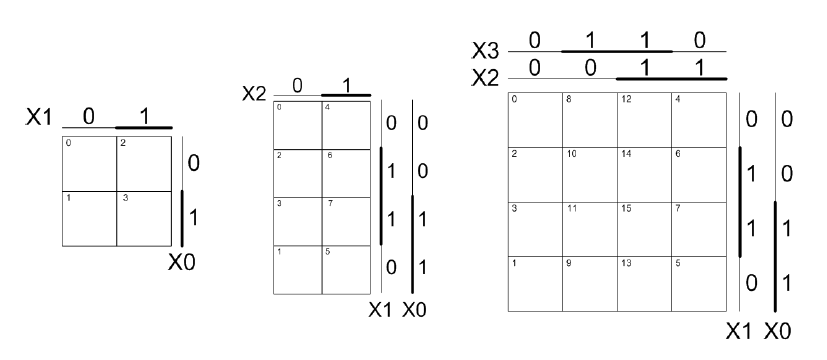
\includegraphics[height=11em]{./Images/DNF-3i-Diagram.png}
\end{minipage}

\noindent\begin{minipage}{\textwidth}
	\textbf{KKNF} - Kanonische konjunktive Normalform - \textbf{Nur 0}\\
	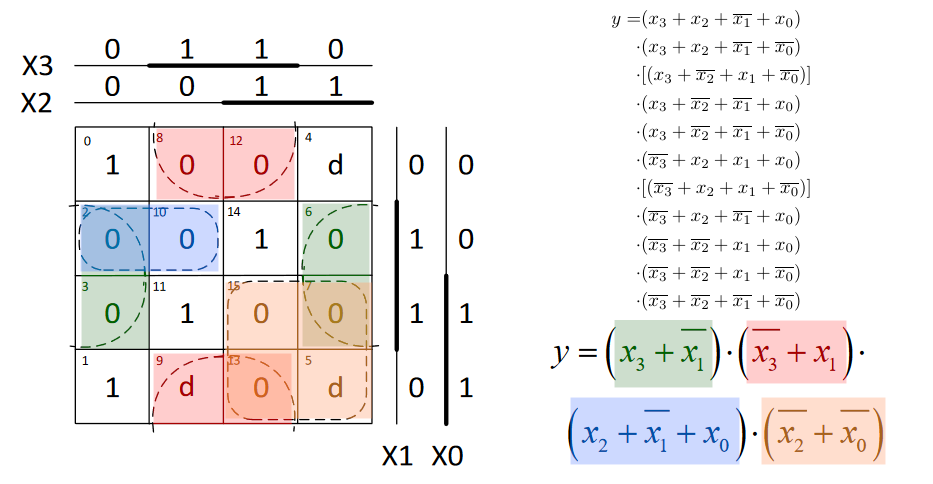
\includegraphics[height=11em]{./Images/KNF-Diagram.png}
\end{minipage}

\noindent\begin{minipage}{\textwidth}
	\textbf{KDNF} - Kanonische disjunktive Normalform - \textbf{Nur 1}\\
	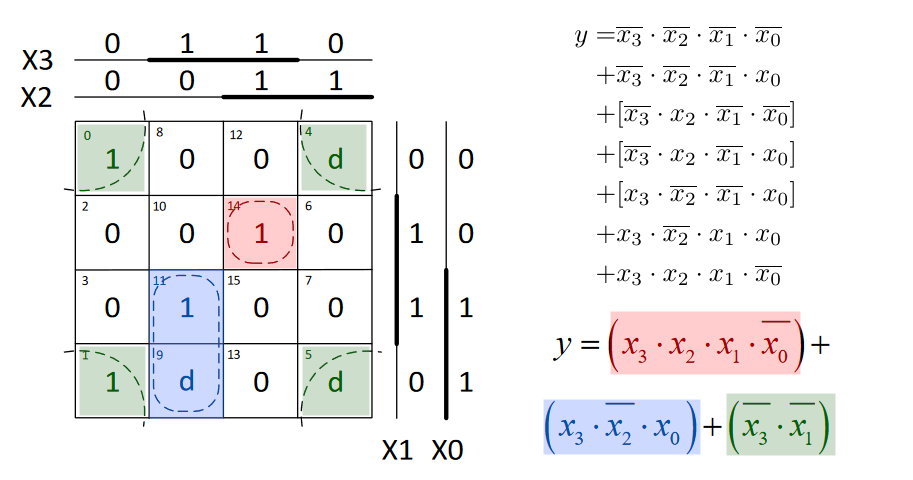
\includegraphics[height=11em]{./Images/DNF-Diagram.png}
\end{minipage}


\section{Logische Gatter}
Die Komplexität einer Schaltung kann mit \textbf{Gatteräquivalents} $n_{ge}$ verglichen werden. \underline{1GE entsprechen 4 Transistoren}. Siehe \verweiseref{symbols}

\subsection{CMOS-Transistor}
Ein CMOS Transistor beinhaltet ein PMOS und ein NMOS Transistor. Dies hat folgende Vor/Nachteile:
\begin{itemize}[nosep]
	\pro kein statischer Stromverbrauch 
	\pro symmetrisches Schaltverhalten
	\pro hohe Störsicherheit
	\pro gebräuchlich und ideale Form für Integration
	\contra mehr Transistoren
\end{itemize}

\noindent
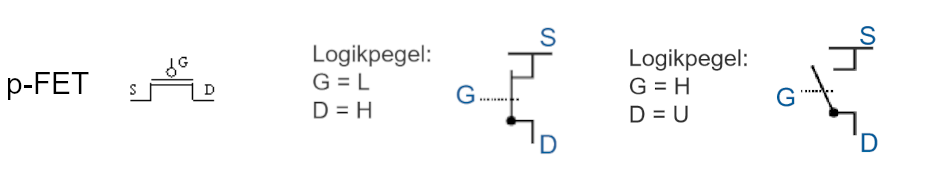
\includegraphics[width=\columnwidth]{./Images/p-fet.png}
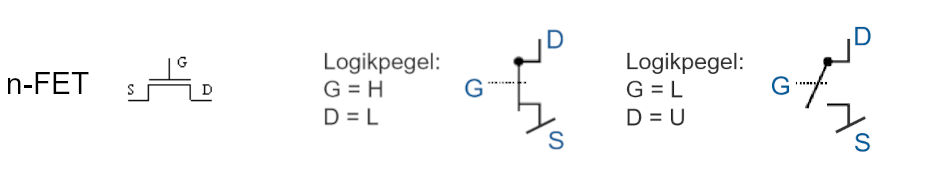
\includegraphics[width=\columnwidth]{./Images/n-fet.png}

\noindent
CMOS-Transistoren dürfen \textbf{NIE} direkt am Ausgang miteinander Verbunden werden (Kurzschluss von VDD nach GND)! Das Verbinden der Eingänge ist erlaubt.

\subsection{Eigenschaften}
\noindent\begin{minipage}{\textwidth}
	\noindent\textbf{Pegelbereich}

	\begin{minipage}{0.25\textwidth}
		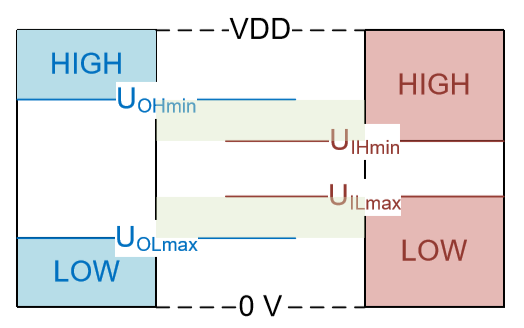
\includegraphics[width=0.8\linewidth,keepaspectratio=true]{./Images/Pegelbereich.png}
	\end{minipage}%%% to prevent a space
	\begin{minipage}{0.25\textwidth}

		\textbf{High-Pegel:}\\ $U_{nH} = U_{OHmin} - U_{IHmin}$ \\
		\textbf{Low-Pegel:}\\ $U_{nL} = U_{ILmax} - U_{OLmin}$
	\end{minipage}
\end{minipage}

\noindent\begin{minipage}{\textwidth}
	\noindent\textbf{Transition Time}
	
	\begin{minipage}{0.25\textwidth}
		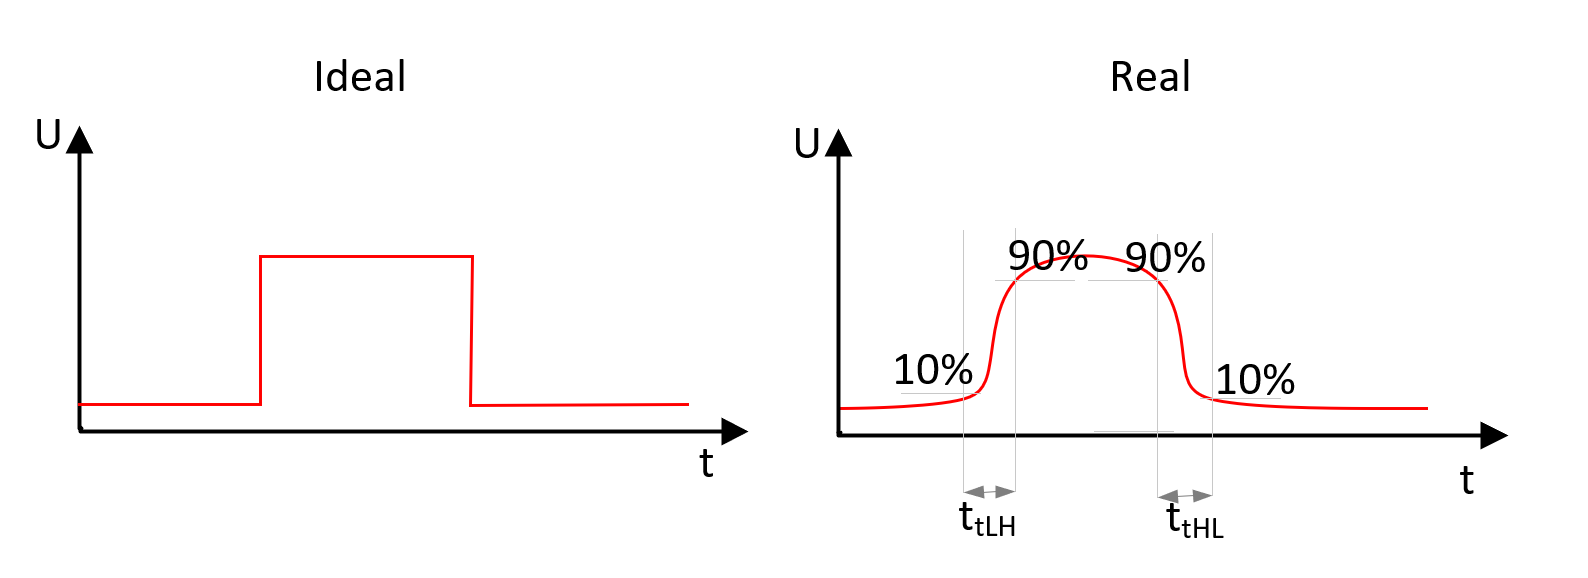
\includegraphics[width=\linewidth,keepaspectratio=true]{./Images/transitiontime.png}
	\end{minipage}%%% to prevent a space
	\begin{minipage}{0.2\textwidth}
		Zeit zwischen 10\% und 90\% von V$_\text{max}$\\
	\end{minipage}
\end{minipage}

\noindent\begin{minipage}{\textwidth}
	\noindent\textbf{Propagation Time}
	
	\begin{minipage}{0.25\textwidth}
		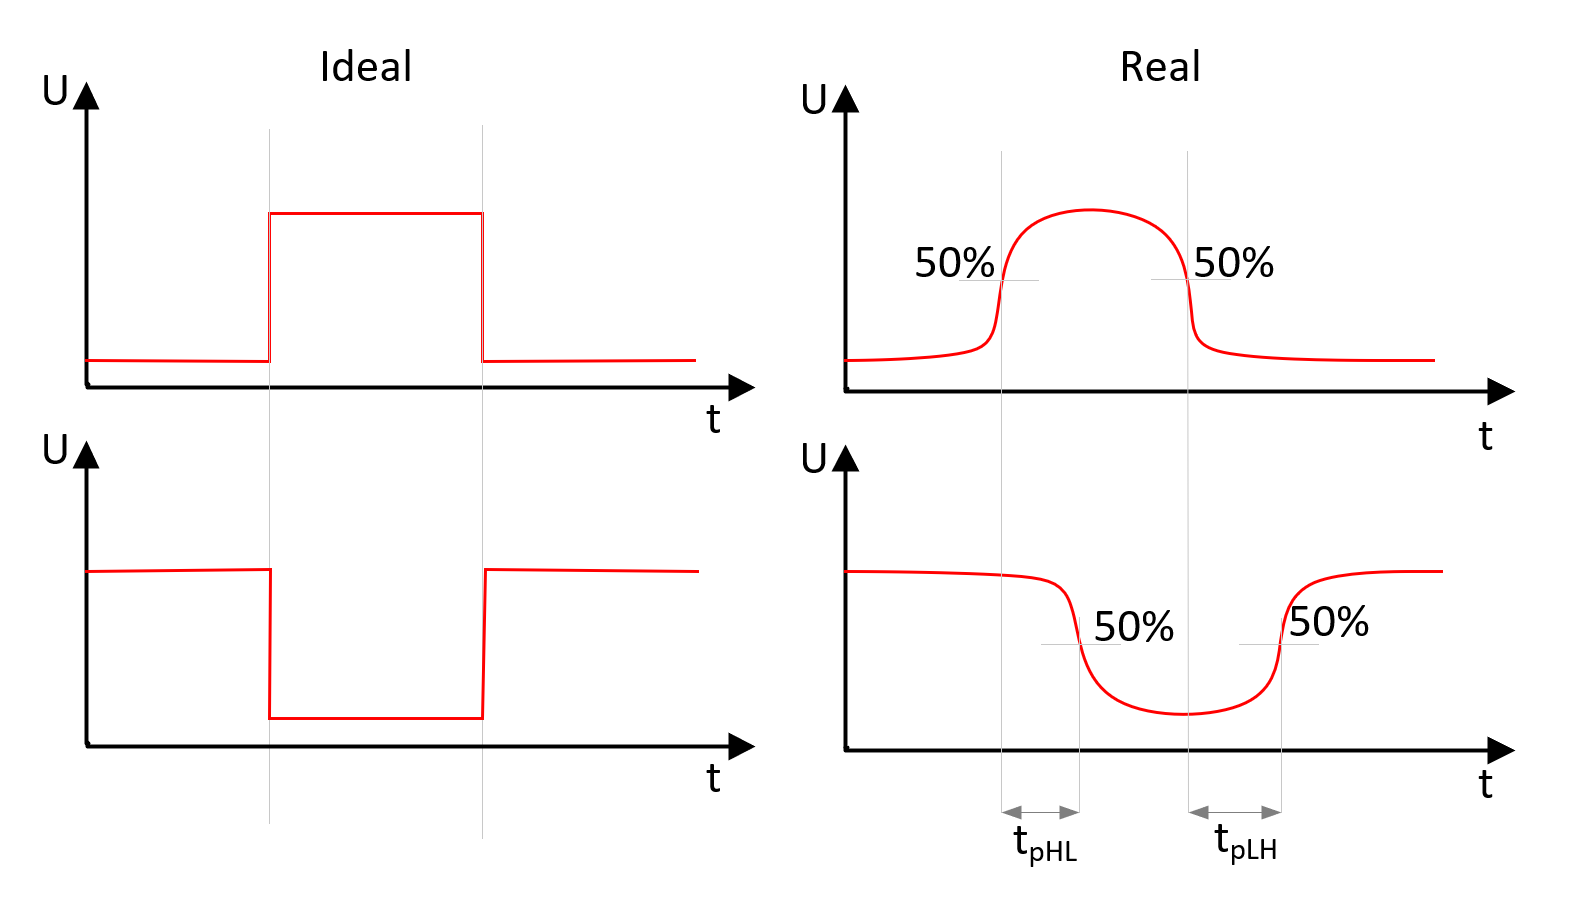
\includegraphics[width=\linewidth,keepaspectratio=true]{./Images/propagationtime.png}
	\end{minipage}%%% to prevent a space
	\begin{minipage}{0.20\textwidth}
		Zeit zwischen 50\% von V$_\text{max}$ Eingang und 50\% von  V$_\text{max}$ am Ausgang
	\end{minipage}
\end{minipage}


\noindent\begin{minipage}{\textwidth}
	\noindent\textbf{Propagation Time}
	
	\begin{minipage}{0.2\textwidth}
		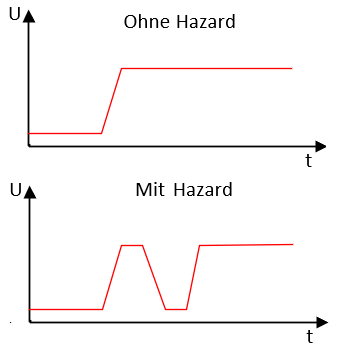
\includegraphics[width=\linewidth,keepaspectratio=true]{./Images/hazard.png}
	\end{minipage}%%% to prevent a space
	\begin{minipage}{0.25\textwidth}
			Bei \textbf{statischen}-Hazards ändert sich der Pegel einmalig, obwohl die Eingänge gleichbleibend sind. \textbf{Dynamische}-Hazards ändern Pegel mehrmalig.
	\end{minipage}
\end{minipage}


\section{Sequenzielle Schaltung}
\textbf{Kombinatorische} Schaltungen sind Zustandsfrei. Ausgänge sind direkt von Eingängen abhängig.\\
\textbf{Sequenzielle} Schaltungen sind zustandsbehaftet (d.h. mehrere Zustände). Vergangenes Verhalten und Eingänge bestimmen momentanen Zustand und Ausgänge.

\subsection{Takt}
\begin{tabular}{ll}
	Periode & $T = T_{on} + T_{off}$ \\
	Frequenz &  $F = \frac{1}{T}$ \\
	DutyCycle &  $DutyCycle = \frac{T_{on}}{T}$ \\
\end{tabular}

\subsection{Synchron/Asynchron}
Bei \textbf{Synchron} wechselt der Zustand bei einer Flanke des Clocks statt.\\
Bei \textbf{Asynchron} kann der Zustand zu jeder Zeit statt finden.

\subsection{Hardware Grundelemente}
\todo{TODO}
\begin{itemize}[nosep]
	\item RS-Latch
	\item D-Latch
	\item D Flip-Flop
	\item Master Slave Flip-Flop
\end{itemize}

\subsection{Timing Diagram - Längster Pfad}
\begin{minipage}{\columnwidth}
	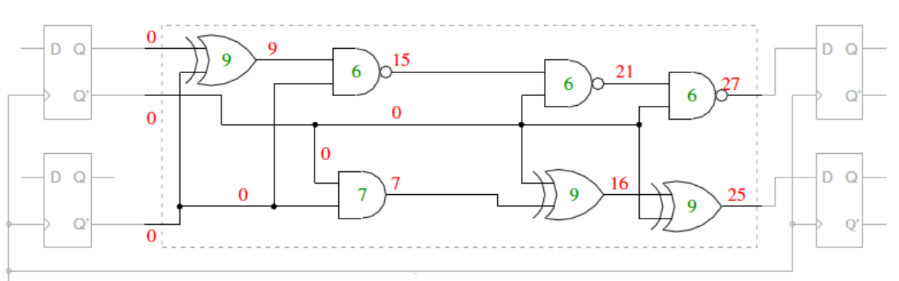
\includegraphics[width=\columnwidth,keepaspectratio=true]{./Images/pfad.png}\\
	Eingänge mit $0$ beschriften, anschliessend recursive alle Ausgänge = $\max\{\text{Eingänge}\} + t_p$. Der längste Pfad ist $\max\{\text{Eingänge}\}$.
\end{minipage}
\section{Sequenzielle Systeme}
\subsection{Zustandstabelle}
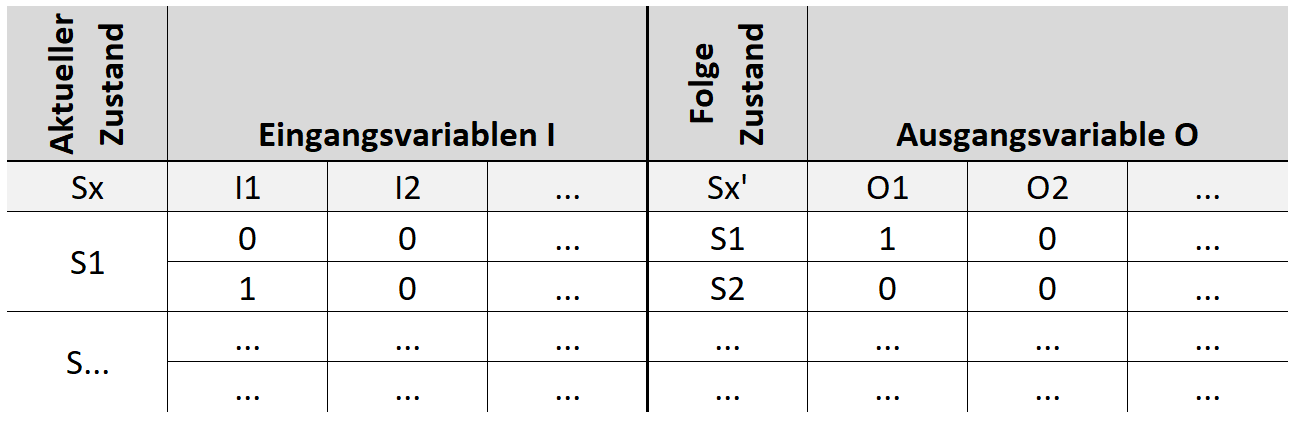
\includegraphics[width=\columnwidth,keepaspectratio=true]{./Images/zustandstabelle.png}

\subsection{Zustandsdiagramm}
\begin{minipage}{\textwidth}	
	\begin{minipage}{0.25\textwidth}
		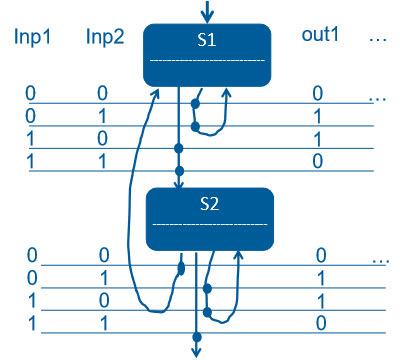
\includegraphics[width=\linewidth,keepaspectratio=true]{./Images/zustandsdiagram.png}
	\end{minipage}%%% to prevent a space
	\begin{minipage}{0.25\textwidth}
		\begin{enumerate}
			\item Zustände zeichnen 
			\item Initial Zustand bestimmen
			\item Eingänge systematisch auflisten
			\item Zustandsübergänge bestimmen
			\item Ausgänge einzeichnen
		\end{enumerate}
	\end{minipage}
\end{minipage}

\subsection{Zustandscodierung}
\noindent\textbf{Binär Codierung}\\
Kompakt und weniger FlipFlop als One-Hot/Cold.

\begin{tabular}{ll}
Anzahl Speicherstellen $k$:& $k = \lceil\ln(p)\rceil = \left\lceil \frac{\log_{10}(p)}{\log_{10}(2)}\right\rceil$\\
maximale Anzahl Zustände $p$:& $p <= 2^k$ \\
Möglichen Zustandscodierungen $q$:& $q = \frac{(2^k)!}{(2^k - p)!}$ 
\end{tabular}\\ 

\noindent\textbf{Gray Code}\\ 
Spezialfall von Binärcodierung, es wechselt jeweils nur 1 Bit zwischen den Zuständen. \\

\noindent\textbf{One-Hot/Cold Codierung}\\
One-Hot (alles 1), One-Cold (alles 0) sind schneller als Binär-Codierungen.

\begin{tabular}{ll}
	Anzahl Speicherstellen $k$:& $k = p$\\
	maximale Anzahl Zustände $p$:& $p = k$ \\
	Möglichen Zustandscodierungen $q$:& $q = p!$ 
\end{tabular}

\section{Finite State Machine (FSM)}
\subsection{Typen}
\noindent\textbf{Mealy-System}: Wert der Ausgänge ist von Eingängen und Zuständen Abhängig. Eingänge gehen asynchron durch. Kann zu \underline{Timing Problemen} führen!

\noindent\textbf{Moore-System}: Wert der Ausgänge ist nur vom aktuellen Zustand des Systems abhängig.

\noindent\textbf{Medwedjew-System}: Spezialfall des Moore-Systems: Ausgänge entsprechen dem Zustandsvektor. \\

\subsection{Timing}
\begin{minipage}{\columnwidth}	
	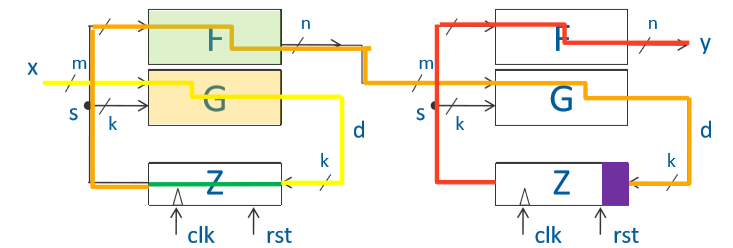
\includegraphics[width=0.8\columnwidth,keepaspectratio=true]{./Images/timingff.png}\\

	$t_{max}$ = \textcolor{green}{Propagation-Delay FF1} + \textcolor{orange}{längster Pfad von F und G Block} + \textcolor{violet}{Setup-Time FF2}. ($f \leq \frac{1}{t_{max}}$)

\end{minipage}
\\ \\
\noindent Timing von Mealy-System können nicht berechnet werden, da diese Asynchrone Anteil haben.
\newpage 
\begin{landscape}
    \section{Symbols}\label{symbols}
    \begin{center}
        \includegraphics[width=\linewidth]{./Images/Übersicht.png}
    \end{center}
\end{landscape}

\end{document}